\documentclass[bsc,frontabs,twoside,singlespacing,parskip,deptreport]{infthesis}

\usepackage[round]{natbib}
\usepackage[hidelinks,colorlinks,allcolors=blue]{hyperref}

\usepackage{graphicx}

\usepackage{textcomp} % for text tilde

% Nice references including the words Figure, Section, etc
\renewcommand*{\chapterautorefname}{Chapter}
\renewcommand*{\sectionautorefname}{Section}
\renewcommand*{\subsectionautorefname}{Section}
\renewcommand*{\figureautorefname}{Fig.}
\renewcommand*{\tableautorefname}{Tab.}
\newcommand{\algorithmautorefname}{Alg.}
\renewcommand{\equationautorefname}{Eq.}

% Change font family and size in captions
\DeclareCaptionFont{captionfont}{\small\fontseries{n}\fontfamily{phv}\selectfont}
\captionsetup[table]{labelsep=period,font=captionfont,justification=centering}
\captionsetup[figure]{labelsep=period,font=captionfont,justification=centering}


%
% TABLES
%

\usepackage{multirow} % multi-row and multi-column table cells
\usepackage{makecell} % line breaks inside cells with \thead{} and \makecell{}
\usepackage{longtable} % allow table to span multiple pages

% Globally setting the vertical padding in tables
\renewcommand{\arraystretch}{1.1}

% Spacing around lines in tables
\def\abovestrut#1{\rule[0in]{0in}{#1}\ignorespaces}
\def\belowstrut#1{\rule[-#1]{0in}{#1}\ignorespaces}
\def\abovespace{\abovestrut{0.17in}}
\def\aroundspace{\abovestrut{0.17in}\belowstrut{0.10in}}
\def\belowspace{\belowstrut{0.10in}}


% For minipages with multiple figures, each with its own subcaption
\usepackage{subcaption}

\begin{document}

\title{\vspace{-5.0cm} \centering{\includeshield} \vspace{1cm} \\ Teacher-student knowledge distillation from BERT\\for sentence classifiers}

\author{Sam Su\v{c}\'ik}

\course{Master of Informatics}
\project{\vspace{3cm}{\bf MInf Project (Part 2) Report}}

\date{2020}

\abstract{
  
}

\maketitle

\section*{Acknowledgements}{
  I thank Steve Renals of University of Edinburgh and Vova Vlasov of Rasa for supervising me throughout the academic year; patiently listening to my never-ending reports and providing helpful and optimistic comments.

  Many thanks also to Ralph Tang whose work inspired this project, and to Sl\'avka He\v{z}elyov\'a who constantly supported me and motivated me to explain all of my work in non-technical stories and metaphors.
}

{
  \hypersetup{linkcolor=black}
  \tableofcontents
}

\chapter{Introduction}{
  % what's the problem, 
  \section{Motivation}{
    \begin{itemize}
      \item After the deep learning hype started, NLP went through an era of LSTMs. Since 2017, the area has been becoming dominated by Transformer models pre-trained on large unlabelled corpora.
      
      \item As newer and bigger Transformer-based models were proposed in 2018 and 2019, improving on the SOTA, it was becoming clearer that their big size and low speed was rendering them difficult to use (both train and deploy) in practice outside of research labs.
      
      \item Recently, we've seen various early attempts at making Transformers -- in particular BERT \citep{Devlin_2018} -- smaller by removing attentional heads \citep{Michel_2019}, quantisation and pruning \citep{Cheong_2019, Sucik_2019}. In terms of actually down-sizing and accelerating the models, knowledge transfer using teacher-student knowledge distillation has led to the most attractive results \citep{Mukherjee_2019,Tang_2019a,Jiao_2019,Sanh_2019}.
      
      \item However, these studies focus only on using knowledge distillation as a tool. Important questions about the nature of this technique and how it interacts with properties of the teacher and student models remain generally unexplored.
      
      \item In line with the increasing demand for explainable AI, it is desirable that, for the beginning, at least the researchers better understand the tools they use, in this case distillation of NLP knowledge from Transformer models. Indeed, such understanding is also useful for overcoming the limitations and designing new variants of this method for smaller and better classifiers.
    \end{itemize}
  }
  
  % what I tried to address, 
  \section{Aims}{
    I aim to better understand knowledge distillation by exploring its use for knowledge transfer from BERT into different student architectures on various NLP tasks.

    This can be further broken down into three aims:
    \begin{itemize}
      \item Explore the effectiveness of knowledge distillation in very different NLP tasks. To cover a broad variety of tasks, I use sentence classification datasets ranging from binary sentiment classification to 57-way intent classification to linguistic acceptability.
      \item Explore how distilling knowledge from a Transformer varies with different student architectures. I limit myself to using the extremely popular BERT model \citep{Devlin_2018} as the teacher architecture. As students, I use two different architectures: a BiLSTM, building on the successful work of Ralph Tang \citep{Tang_2019a,Tang_2019b}, and a down-scaled BERT architecture.
      \item Explore how successfully can different types of NLP knowledge and capabilities be distilled. Since NLP tasks are often possible for humans to reason about, I analyse the models' behaviour (e.g. the mistakes they make) to learn more about knowledge distillation. I also probe the models for different linguistical capabilities, inspired by previous successful probing studies \citep{Conneau_2018,Tenney_2019b}.
    \end{itemize}
  }
  
  % what I did
  \section{Contributions}{
    My actual findings. To be added later.
  }
}

% Prerequisites: define NLP abbreviation
\chapter{Background}{
  \label{ch:background}

  In this chapter, the Transformer models are introduced and set into the historical context; knowledge distillation is introduced, in particular its recent applications in NLP; and an overview of some relevant work in model understanding is given.

  % NLP (sentence classification), transformers, knowledge distillation, model understanding (probing)
  \section{NLP before Transformers}{
    \label{sec:pre-transformer-nlp}
    % NLP is all about sequences of variable lengths: sentences, sentence pairs, documents, speech segments...
    By the very nature of the natural language, its processing has always meant processing sequences of variable length: be it written phrases or sentences, words (sequences of characters), spoken utterances, sentence pairs, or entire documents.
    % NLP tasks are typically about making simple predictions about sequences: classifying sentences based on their intent or language, scoring a document's level of formality, predicting whether two sentences form a coherent question-answer pair or not, predicting the next word of a sentence...
    Very often, NLP tasks boil down to making simple decisions about such sequences: classifying sentences based on their intent or language, assigning a score to a document based on its formality, deciding whether two given sentences form a meaningful question-answer pair, or predicting the next word of an unfinished sentence.

    % Machine learning predictors are typically designed to work with fixed-size representations of inputs. Therefore, ever since the resurgence of neural networks around 2010, neural NLP has been using various models for encoding variable-length sequences into common fixed-dimensional representations.
    Machine learning models are typically suited for tasks where the dimensionality of inputs and outputs is known and fixed. Thus, natural language sequences as inputs pose a challenge. It comes as no surprise that NLP research has been focusing on developing models that can encode variable-length sequences into fixed-length representations. 
    \textbf{(TO-DO: Maybe mention TDNNs? They kind of fit here although they process speech, not text...)}
    For example, once any sentence can be embedded as a vector in a space with a fixed dimensionality, a simple sentence classification model can be learned on top of these vectors.

    % Word vectors used already by \citet{Collobert_Weston_2008,Collobert_Weston_2011}, trained in unsupervised fashion. Used for various NLP tasks in a CNN.
    As early as 2008, Collobert and others \citep{Collobert_Weston_2008,Collobert_Weston_2011} introduced a key component of today's sequence encoder models: the idea of \textit{word embeddings}, i.e. rich, fixed-length representations of words, constructed to numerically encode various word properties (e.g. lexical, syntactical or semantical). When viewed as a lookup table (one vector per each supported word), the embeddings are used to ``translate'' input words into numerical vectors. These are then further processed by a model.
    % Word2vec \citet{Mikolov_2013} made embedding learning much more efficient (and made learning the embedings the main aim!), using CBOW and skip-grams.
    \citet{Mikolov_2013} introduced an efficient and improved way of learning high-quality word embeddings: \textit{word2vec}. The embeddings are learnt as part of a larger neural network, which is trained to predict the next word given several previous words, and the previous words given the current word\footnote{These are the so-called Continuous bag-of-words (CBOW) and Skip-gram (SG) tasks, respectively.}. Such training can be easily done on large amounts of unlabelled text data, and the embeddings learn to capture various properties from a word's morphology to its meaning. Released word2vec embeddings became very popular due to their ease of use and performance improvements in many NLP tasks.

    RNN- and later LSTM-based encoder architectures were dominating the area for a long time as they were naturally suited for processing sequences of any length.

    A major breakthrough came when \citet{Kalchbrenner_2013} and \citet{Sutskever_2014} developed the encoder-decoder architecture for machine translation and other sequence-to-sequence tasks such as paraphrasing or parsing.

    \citet{Bahdanau_2014} improved things by introducing attention, enabling the recurrent encoders to learn to selectively attend or ignore parts of the input sequence.
  }

  \section{Transformer models and BERT}{
    \citet{Vaswani_2017} introduced Transformer. Main idea: process tokens in parallel, not sequentially, with sequentiality represented by positional markers (embeddings). Self-attention is used to pool from the context of the entire sequence, leading to evolving rich contextualised representations of each token in the higher layers.
    
    \citet{Radford_2018} introduced the idea of generative LM pre-training and fine-tuning. This concept helps train much better models even for low-resource tasks with small datasets, by leveraging general language knowledge acquired by the model in the pre-training phase. Publishing pre-trained model instances makes the power of NLP much more accessible to anyone and has become a popular thing to do. (Also mention that subword tokens were used instead of words.)
    
    \citet{Devlin_2018} improved the concept by pre-training the model bi-directionally (leading to language modelling based on left \textit{and} right context). They also changed the pre-training to 2 tasks trained at the same time: masked language modelling to learn to understand words, and next sentence prediction to learn to reason about entire sentences (as the actual NLP tasks often require such reasoning). This is is how BERT was born, which then became extremely popular in the community, attracting a lot of work on improving it, analysing its capabilities, extending it to other languages, and even applying it to multi-modal tasks such as video captioning. TO-DO: elaborate more on BERT, also with a schematic picture.
    
    Following the success of BERT, further and often bigger Transformer models started emerging:
    \begin{itemize}
      \item GPT-2 \citep{Radford_2019}, a bigger and improved version of GPT
      \item XLM \citep{Lample_2019} with added introduced cross-lingual pre-training
      \item Transformer XL \citep{Dai_2019} with better handling of much longer contexts
      \item and many others
    \end{itemize}

    Although the open-sourced powerful pre-trained models were a huge step towards more accessible NLP, the model size meant they couldn't be applied easily outside of research: They were memory-hungry and slow. 
    This inspired another wave of research: compressing the huge, well-performing Transformers (very often BERT) to make them faster and resource-efficient. 
    I will focus on the compression method that so far looks the most effective: knowledge transfer from huge models into smaller ones using teacher-student knowledge distillation.
  }

  \section{Teacher-student knowledge distillation}{
    % brief history of KD in general
    % different objectives: logits, hard labels, mimicking internal representations...
    \subsection{Brief history of knowledge distillation}{
      The concept of knowledge distillation was introduced by \citep{Bucila_2006} as a way of knowledge transfer from huge models (or ensembles of models) into small ones, with the aim of having smaller (and hence faster) yet well-performing models.
      The main idea is to train a big neural classifier model also called the \textit{teacher} and then let a smaller neural classifier model (called the \textit{student}) learn from it -- by learning to mimic the teacher's behaviour. Hence also the term \textit{teacher-student knowledge distillation}.
      The mimicking was originally realised by labelling a dataset with the trained teacher model and training the student model on these labels (retrospectively referred to as \textit{hard labels}). The dataset used for training the student model is often called the \textit{transfer dataset}.

      Later, \citet{Ba_2013} introduced the idea of learning from the \textit{soft labels}, i.e. learning to predict the teacher's logits. The idea is that the teacher's knowledge can be transferred to the student in a richer way if the entire logit distribution is utilised (compare with hard labels, when only the information about the maximum element of the logit distribution is utilised). When first proposed, the student's loss function was then mean squared distance between the student's outputs and teacher's logits.

      \citet{Hinton_2015} proposed a more general approach, addressing the issue of overconfident teachers with very sharp logit distributions, and formulated a new loss for student models: the cross-entropy loss with temperature. The temperature softens the teacher's sharp distribution, allowing the student to learn more rich information from it. This approach is what is today typically referred to as knowledge distillation.

      Since 2015, further variants have been proposed, enhancing knowledge distillation in different ways, for example:
      \begin{itemize}
        \item \citet[p. 13]{Papamakarios_2015} points out that mimicking teacher outputs (e.g. with cross-entropy loss) can be extended to mimicking the derivatives of the loss w.r.t. inputs (i.e. including in the loss function also this term: $\frac{\partial \mathbf{o}_{student}}{\partial \mathbf{x}} - \frac{\partial \mathbf{o}_{teacher}}{\partial \mathbf{x}}$). %, the additional loss term being calculated using the R technique (Pearlmutter, 1994).
        \item \citet{Romero_2015} introduced the idea of learning to match not just the teacher's outputs, but also its intermediate input representations. \citet{Huang_2017} achieved this by learning to align the distributions of neuron selectivity patterns between the teacher's and student's hidden layers. Unlike standard knowledge distillation, this approach no longer works just for classifier models with a softmax output layer (see the standard loss proposed by \citet{Hinton_2015}).
        \item \citet{Sau_2016} show that learning can be more effective when noise is added to the teacher logits.
        \item \citet{Mirzadeh_2019} show that a knowledge distillation performs poorly from large teachers into very small students and alleviate this limitation by multi-stage distillation: first distilling knowledge into an intermediate-size ``teacher assistant'' and learning the student from the assistant model.
      \end{itemize}
    }

    \subsection{Knowledge distillation in NLP}{
      % \citet{Kim_2016} observe that KD and weight pruning are orthogonal (can be used together), and that mimicking top-most hidden layer outputs (instead of outputs themselves) doesn't provide improvements previously reported.
      Practically all the so far mentioned research in knowledge distillation was done in the domain of image processing. This comes as no surprise: It was image processing that was benefitting the most from the resurgence of deep learning. Ever since the AlexNet \citep{Krizhevsky_2012}, bigger and bigger models were proposed, simultaneously driving the research in model compression so as to make the models usable in practice.

      % KD in NLP: sequence-level KD \citep{Kim_2016}, then basically straight to distilling from BERT?
        % In the NLP literature, it has previously been used in neural machine translation (Kim and Rush, 2016) and language modeling (Yu et al., 2018).
      In natural language processing, research on knowledge distillation was rare for a long time. One notable work was the adaptation of distillation for sequence-to-sequence machine translation models -- whose outputs are no longer simple classification scores -- by \citet{Kim_2016}. Another pioneering study compressed a recurrent neural language model for use on mobile devices \citep{Yu_2018}.

      However, the real need for model compression started very recently when huge Transformer models were introduced. This follows on from the main limitation of the otherwise very accessible pre-trained models: being huge and slow.

      When distilling knowledge from big, pre-trained Transformer models, the main decision is whether to distil before or after fine-tuning on a concrete downstream task. Each option has its pros and cons.
      In the first scenario, the steps are: 1) distilling into a small student, 2) fine-tuning the student on any downstream task. One advantage is that the distillation is done only once and fine-tuning the student can be fast (due to the student's size). Since the distillation can be done on the same data that the teacher was pre-trained on -- large corpora of unlabelled data, one does not have to worry about not having enough data. One possible downside is that the amount of general language knowledge contained in the pre-trained teacher will be too much to contain within a small student, hence requiring students that are themselves considerably large (and slow). \citet{Sanh_2019} took this approach and while their student model is very successfully fine-tuned to a wide range of tasks, it smaller than the teacher (BERT base) only by 40\%, still having 66M parameters.
      % Distilling beforeinto a small student and subsequently finetuning it on any downstream task means easy 
      %   pros: have flexible model that's easy to finetune for any downstream task. lots of transfer data to work with.
      %   cons: too small model may not be able to take all of teacher's useful knowledge
      %   Sanh tried and only got to making BERT 60\% smaller??? (# of params).

      % CAREFUL NOT TO MIX IN OWN METHODOLOGY HERE!!!
      In the second scenario, the steps are: 1) fine-tuning the pre-trained teacher on a downstream task, 2) distilling the teacher into a small student. 
      In this case, the downstream task-specific language knowledge is likely to be much smaller than the teacher's overall pre-trained language knowledge, meaning that a much smaller student can still contain all important knowledge from the fine-tuned teacher. 
      However, with this approach, the teacher fine-tuning and distillation has to be done separately every downstream task, which can be resource-intensive.
      Even more importantly, the distillation procedure can suffer from lack of data, since the distillation is now being done only with the downstream task dataset, which will often be small and has to be augmented.
      Various ways of augmenting small datasets to increase the amount of transfer data have been proposed, with mixed success. 
      \citet{Mukherjee_2019} use additional unlabelled in-domain sentences with labels generated by the teacher -- an approach that only works if such in-domain sentences are available. \citet{Tang_2019a} propose augmentation based on simple, rule-based perturbation of existing sentences from the downstream task data. Finally, \citet{Jiao_2019} and \citet{Tang_2019b} use big Transformer models generatively to create new sentences. In the first case, BERT is repeatedly used to choose a suitable replacement for an existing word in a given sentence, eventually leading to a new sentence with many words changed for different ones. In the second case, a GPT-2 model is fine-tuned on the downstream task with a language model objective, and a new sentence is generated by repeatedly predicting the next token, conditioned on the sequence generated so far.
      % After:
      %   pros: only task-specific knowledge is distilled, likely into much smaller model.
      %   cons: have to train big teacher for each downstream task, likely to take long. may need more transfer data than small downstream dataset.
      %   Tang: distilled into much smaller student. didn't address issue of having to train teacher repeatedly. addressed issue of little data quite successfully.

      In this work, I adopt the approach of \citet{Tang_2019b} as I view it as the most promising one so far. However, while they use only bidirectional LSTM students, I also experiment with a smaller version of BERT, similarly to \citet{Jiao_2019}. For detailed description of the system see \autoref{chap:implementation}.
    }
  }
  
  \section{Analysing and understanding NLP models}{
    NNs are black boxes and (not) understanding the models is a serious issue.
    performance is typically more important than transparence, but recently the demand for explainable AI (XAI) has been increasing. additionally, understanding is opportunity for further improvements of the mdels and techniques.

    in image processing, interpretability is easy thanks to visualising things. (somewhat similarly music.) notable works: maximising activation, visualising neurons' output for given input, maximum activation samples.
    in NLP, interpreting is more difficult, and also comes with a delay after image processing -- same with the big model hype and compression hype.
    % hard to do maximising activation or visualising single units. BUT types of information preserved in internal input representations can be well explored: probing!
    \citet{Belinkov_2018} give nice overview of work done up until 2018. they point out that many methods for analysing and interpreting models are adapted from image processing, especially visualising activations of single neurons on specific input examples. in attentional seq2seq models, the attention maps can be visualised to show soft alignments between input and output sequences. however, these methods taken from image processing are mostly qualitative, not suited for comparing models.
    
    more quantitative and NLP-specific are the approaches that look at kinds of linguistic knowledge present in a model's internal representations of input. most often, this means extracting activations for a set of inputs and trying to predict properties of the input from the activations by using a simple predictor model. if the prediction works well, then the activations must've contained linguistic knowledge relevant for the predicted property. since first proposed by \citet{Shi_2016}, this approach has been used repeatedly to explore various forms of representations. the first work was looking at how well NMT systems capture syntactic properties of input. later, \citet{Adi_2017} used simpler artificial prediction tasks (sentence length, word content and word order) to better understand sentence embeddings produced by recurrent encoders. more recently, \citet{Conneau_2018} curated a set of 10 probing tasks ranging from surface properties through syntactic to semantic ones, and compared different recurrent and convolutional sentence encoders (and many useful baseline models) in terms of the linguistic knowledge in their sentence representations.
    focusing specifically on Transformer models, \citet{Tenney_2019a} propose a set of \textit{edge probing} tasks which examine how much contextual knowledge about the entire sentence is captured within the representation of a single word. the tasks mimic the typical steps of a standard NLP pipeline -- from POS tagging to identifying dependencies and entities to semantic role labelling. \citet{Tenney_2019b} were able to localise the layers of BERT that are the most important for each of the tasks, showing that the different linguistic capabilities are ordered within the model in the typical NLP pipeline order: from simple POS tagging in the earlier layers to the most complex semantic tasks in the last layers.

    while the abovementioned methods for analysing models provide valuable insights, they are incomplete. for one, they merely help us describe in intuitive terms the kinds of internal knowledge/specialisation observed in the models. in their overview of interpretability of machine learning, \citet{Gilpin_2018} call this level of model understanding \textit{interpretability} -- comprehending what a model does. however, what we should strive to achieve, is \textit{explainability}: the ability to ``summarize the reasons for neural network behavior, gain the trust of users, or produce insights about the causes of their decisions''. In this sense, today's methods for analysing neural NLP models achieve only interpretability because they enable us to describe but not explain (especially in terms of causality) the internals and decisions of the models.
    
    In this work, I also attempt to mainly \textit{interpret} the student and teacher models. I adopt two approaches:
    \begin{enumerate}
      \item analysing the mistakes the models make on the downstream task they were trained to do, including how confident the correct and incorrect predictions are
      \item probing the models using the probing tasks curated by \citet{Conneau_2018}
    \end{enumerate}
    By comparing the findings between models trained on different downstream tasks or with different architectures, I try to characterise each task in terms of the linguistic capabilities it utilises. 
    Further, I describe how different student model architectures influence how linguistic knowledge is distilled from a teacher and stored in the student, and what the effect on the student's confidence is. 
    Finally, I try to relate the observed effects to the method of knowledge distillation itself.
  }
}

\chapter{Datasets}{
  % GLUE: CoLA, SST-2; Sara (anonymised!), probing tasks. Other alternatives considered.
  \section{Downstream tasks}{
    Since the BERT model I use as teacher is already pre-trained on large unlabelled corpora (for details see the original work by \citet{Devlin_2018}), it can be fine-tuned well even on small downstream datasets.

    Today, perhaps the most popular collection of challenging NLP tasks (challenging by the nature of the tasks and by the relatively small dataset size) is the GLUE benchmark \citep{Wang_2018}. This collection comprises 11 tasks from semantic analysis to detecting textual similarity to natural language inference, framed as single sentence or sentence pair classification. Each task features a specific scoring metric (such as accuracy or F1), publicly available labelled training and development datasets, and a testing dataset whose labels have not been released. The test-set score accumulated over all tasks forms the basis for the popular GLUE leaderboard\footnote{\url{https://gluebenchmark.com/leaderboard}}.
    
    For simplicity, I use only the single-sentence classification tasks of the collection -- the Corpus of Linguistic Acceptability (CoLA) and the Stanford Sentiment Treebank in its two-way classification format (SST-2).
    \begin{itemize}
      \item The CoLA task features 8.5k training sentences, 1k evaluation and 1k testing sentences. The (hand-crafted) sentences are collected from various linguistic literature and represent examples of acceptable and unacceptable English, making the task a binary classification. The scoring metric is Matthew's Correlation Coefficient (MCC, introduced by \citet{Matthews_1975}). This task is rather challenging since a given sentence can be perfectly grammatical and still not be acceptable English. As a non-native speaker, I myself struggle with some of the examples.
      \item The SST-2 task has considerably more data as it is easier to collect: 67k training, 9k evaluation and 18k testing sentences, extracted from movie reviews and labelled as positive or negative sentiment. The scoring metric is accuracy. The task is easier than CoLA and best models in the GLUE leaderboard achieve over 97\% test-set score.
    \end{itemize}

    As the third task, I use an intent classification dataset collected by Rasa, a company building open-source tools for conversational AI\footnote{For transparency: I did a 3-month internship as Machine Learning researcher with Rasa in the summer of 2019.}. The dataset is named Sara, after the company's own chatbot\footnote{Demonstrated at \url{https://github.com/RasaHQ/rasa-demo}} which provides various information about Rasa and its products to the visitors of the company's website\footnote{\url{https://rasa.com/}}. The dataset comprises 4.8k examples overall, split between 1k testing portion and 3.8k training portion. Each example is a human-generated utterance and has been manually labelled with one of 57 intents, helping the Sara chatbot learn to detect what a human is talking to it about. Originally, the dataset was initialised by Rasa employees talking to Sara. Later, many more examples were collected by deploying the chatbot and letting site visitors talk to it. The 57 intent types were designed by Rasa, starting with a smaller number of broader intents and refining the set after observing real questions humans were asking the chatbot. \textbf{TO-DO: verify this is true; my knowledge of the history of Sara is limited.} The main scoring metric is the multi-class micro-averaged F1 score.

    I modified the Sara dataset by splitting the training portion into 2.8k training and 1k evaluation sentences (while keeping both sets class-balanced). I also anonymised the dataset by replacing all sensitive information with generic tokens. Namely, I replaced people's names and surnames with a single token \verb|__PERSON_NAME__| and e-mail addresses with \verb|__EMAIL_ADDRESS__|.

    To stay consistent with the GLUE datasets for which test-set labels are not publicly available, I do not use the test portion of any of them when analysing the mistakes made by different models. Instead, I analyse the predictions on the evaluation set. This can be viewed as sheding light on the kind of model qualities that are actually optimised when choosing model parameters on this set.
  }

  \section{Data augmentation for generating large transfer sets}{
    As \citet{Tang_2019a} demonstrate, taking just the training sentences of a downstream task as the transfer set for knowledge distillation is not enough; especially for challenging tasks like CoLA where the training set comprises only several thousands of sentences (for results, see Table 1 in \citet{Tang_2019b}). I adopt the approach that they found to work the best: Augmenting the training portion with additional sentences generated by a GPT-2 model \citep{Radford_2019}. The concrete steps for this augmentation are:
    \begin{enumerate}
      \item Fine-tune the pre-trained GPT-2 model (the 345M-parameter version) on the training sentences for 1 epoch with the language-modelling objective, i.e. learning to predict the next subword token of a sentence given the true sequence of tokens so far.
      \item Sample a large number of prefixes (subword tokens) from the observed distribution of sentence-initial subword tokens in the training sentences.
      \item For each sampled prefix, generate a sentence starting with it: by sampling from the predicted next-token distribution of the GPT-2 model, starting with just the prefix and stopping when the special end-of-sentence token is generated or the desired maximum sequence length is reached (in this case 128 tokens).
      \item Add the generated sentences to the original training sentences and use as the transfer set, i.e. append with teacher-generated logits and use to train the students.
    \end{enumerate}

    For consistency, I used the same number of augmentation sentences as \citet{Tang_2019a}: 800k for each downstream task. Hence, the transfer set comprises 808.5k sentences for CoLA, 867k sentences for SST-2, and 802.8k sentences for Sara.
  }

  \section{Probing tasks}{
    For exploring the linguistic knowledge in the different teacher and student models, I use the probing task collection curated by \citet{Conneau_2018}.
    The datasets, along with tools for applying probing to neural models, are publicly available as part of the SentEval toolkit \citet{SentEval-paper} for evaluating sentence representations.
    The collection contains 10 tasks, each having 100k training, 10k evaluation and 10k testing sentences. These are used for training the probing classifier, choosing its hyperparameters, and computing the task-specific score, respectively.

    Each of the 10 probing tasks -- grouped into three broad categories -- focuses on a different linguistic capability (for more details, see the original paper of \citet{Conneau_2018}):
    
    Surface information:
    \begin{itemize}
      \item \textbf{Length} is about recovering the length of the sentence. The actual sentence lengths are grouped into 6 equal-width bins, making this task a 6-way classification.
      \item \textbf{WordContent} is about identifying which words are present in the sentence. A collection of 1000 mid-frequency words was created, and sentences were sampled such that each contains exactly one of these words. The task is therefore 1000-way classification.
    \end{itemize}
    Syntactic information:
    \begin{itemize}
      \item \textbf{Depth} is about classifying sentences by their syntactic parse tree depth, with depths ranging from 5 to 12 (hence 8-way classification).
      \item \textbf{BigramShift} is about recognising sentences in which the order of two randomly chosen adjacent words has been swapped (binary classification).
      \item \textbf{TopConstituents} is about recognising the top syntactic constituents -- the nodes found in the syntactic parse tree just below the S (sentence) node. This is framed as 20-way classification, choosing from 19 most common top-constituent sequences and the ``other'' option.
    \end{itemize}
    Semantic information:
    \begin{itemize}
      \item \textbf{Tense} is binary classification, identifying the tense (present/past) of the main verb of the sentence (the verb in the main clause).
      \item \textbf{SubjNumber} is about determining the number (singular/plural) of the sentence's subject, framed as binary classification.
      \item \textbf{ObjNumber} is the same as SubjNumber, applied to the direct object of a sentence.
      \item \textbf{OddManOut} is binary classification, detecting whether a random word (verb or noun) in a sentence was replaced with a different one (verb or noun) or not. To make this task more difficult, the replacement word is chosen such that the frequency of the bigrams in the sentence stays roughly the same.
      \item \textbf{CoordinationInversion} works with sentences that contain two coordinate clauses whose order may have been artificially swapped. The binary classification is then about detecting which sentences are intact.
    \end{itemize}

    Considering the findings of \citet{Tenney_2019b} about the NLP pipeline steps being implicitly captured inside BERT, choosing their approach to probing (together with the collection of tasks they curated) was an attractive option. However, the approach explores single-word representations, focuses primarily on more complex probing tasks (e.g. entity recognition, natural language inference, semantic roles) and the tasks are not open-sourced. In this sense, the SentEval toolkit is preferred as it was built for analysing sentence representations, the simpler surface and syntactic tasks have a better coverage, and the datasets are publicly available. In the future, however, the two collections of probing tasks could be used in combination.
  }
}

\chapter{Implementation}{
  \label{chap:implementation}
  % pytorch-transformers, d-bert, SentEval, Rasa. own pieces. architecture. choices made. initial hparams.
  \section{Existing implementations used}{
    For finetuning BERT, I used \verb|transformers| \citep{Wolf_2019}\footnote{\url{https://github.com/huggingface/transformers}, accessed January 30, 2019} -- a popular open-source PyTorch library curating and presenting many successful Transformer-based models in a unified way.
    My implementation of the distillation process is heavily based on the implementation accompanying DistilBERT \citep{Sanh_2019}, which is today part of \verb|transformers|\footnote{\url{https://github.com/huggingface/transformers/tree/master/examples/distillation}, accessed January 30, 2019}.

    The implementation of the BiLSTM student is based on the codebase accompanying the work of \citet{Tang_2019b}\footnote{\url{https://github.com/castorini/d-bert}, accessed January 30, 2019} (which was originally built using an early version of the \verb|transformers| library). The same codebase was used without many changes for fine-tuning the GPT-model and creating the augmentation sentences.

    Finally, for probing, I adapted the SentEval toolkit \citep{SentEval-paper} to suit my needs.

    In terms of implementation, the most of my own work is in having integrated the different tools. In particular, I have combined the codebases of \citet{Sanh_2019} and \citet{Tang_2019b} and adapted the combination to offer richer options (e.g. initialising the student's embedding layers with trained word or wordpiece embeddings), to work with both BERT and BiLSTM students and to be more easily extendable to other architectures.
  }
  \section{System overview}{    
    Following \citet{Tang_2019b}, I used the large, case-insensitive (uncased) pre-trained BERT (340M params) as the teacher and finetuned it for 3 epochs using Adam optimizer with $\eta=5e-5$ with linear warm-up over the first 10\% of training steps, followed by linear decay, and with batch size $B=36$. I will refer to this model as $BERT_T$. Somewhat surprisingly, while the teacher converged within 3 epochs for CoLA and SST-2 (in terms of the dev-set score), for Sara, it converged much more slowly. I empirically chose 10 epochs as the smallest number after which $BERT_T$ would sufficiently converge on the Sara dataset.

    As students, I used:
    \begin{itemize}
      \item a bi-directional LSTM same as the one used by \citet{Tang_2019b}: with one LSTM layer with 300 units, followed by a linear layer with 400 units and ReLU activation function, with a softmax classifier on top, with 2.41M non-embedding trainable parameters. I will refer to this model as $LSTM_S$.
      \item a smaller version of the teacher BERT model, with all dimensions down-scaled 5x to roughly match the number of trainable non-embedding parameters: with 5 transformer layers, hidden dimension of 204, intermediate layers of size 750, and 3 attentional heads (amounting to 2.42M parameters). I will refer to this model as $BERT_S$.
    \end{itemize}

    $LSTM_S$ was trained to minimise the mean squared loss (MSE) between the teacher-generated logits and student's logits. While the cross-entropy loss with configurable temperature is more popular and in essence a generalisation of the MSE loss (see \citet{Hinton_2015}), \citet{Tang_2019b} report that the MSE loss led to slightly better performance in their experiments. For $BERT_S$, I use the traditional cross-entropy loss with temeperature set to $T=3$ following the findings of \citet{Tsai_2019} who experimented with different temperatures (note that $T=3$ was used as the default also in the experiments of \citet{Tang_2019b}).

    Following preliminary experiments, I limited the number of training epochs to 30 for $LSTM_S$ (same budget was used by \citet{Tang_2019b}) and to 60 for $BERT_S$ as it was converging much slower than the recurrent student. I stick to this training budget throughout my experiments.

    some overall visualisation of all the components and how they interact
  }
}

\chapter{Student tuning}{
  Importantly, extensive tuning of the students' hyperparameters is certainly not the main objective of this work. However, my aim is to carry out an analysis of the teacher and student models and the distillation process. For such analysis to be of some value, it should be done using well-performing models which themselves are of practical value.

  I tune a number of hyperparameters for the 2.4M-parameter students using the CoLA task. Afterwards, I tune a smaller number of parameters -- which are the most likely to be task-dependent -- separately for each downstream task, trying to obtain $LSTM_S$ and $BERT_S$ that would achieve 90\% of the teacher's performance while being as small as possible. These student are then used for further analysis.

  For both students, I first tune the following, in this order (for more details, see the next sections):
  \begin{enumerate}
    \item learning rate $\eta$
    \item learning rate scheduling, more concretely the warm-up and decay of $\eta$
    \item batch size $B$
    \item embedding type (wordpiece vs word) and mode
  \end{enumerate}

  Afterwards, I tune on each task separately the embedding type and the student size.

  The starting configuration (which I change as I tune the different parameters) is:
  \begin{itemize}
    \item $BERT_S$: Adam with $\eta=5e-5$, $B=256$, learning rate warm-up over the first 10 epochs, followed by linear decay, and wordpiece embedding layer
    \item $LSTM_S$: Adadelta with $\eta=1.0$, $B=50$, no learning rate annealing, and word embedding layer in the multichannel mode, using word2vec
  \end{itemize}
  Initially, $LSTM_S$ had its embedding layer initialised with word2vec embeddings, but $BERT_S$ was initialised entirely from scratch. Naturally, this was posing a disadvantage for $BERT_S$ as it was starting with no knowledge. Hence, I added the option to initialise the embedding layer with wordpiece embeddings from the corresponding finetuned $BERT_T$. I report results of parameter tuning for both of these variants of $BERT_S$.
  
  \section{Choosing $\eta$}{
    Because \citet{Tang_2019b} report not tuning their hyperparameters, I acknowledge their parameter choices but challenge many of them. In particular, they use Adadelta with $\eta=1.0$ and $\rho=0.95$ as the learning algorithm. I attempt to use the Adam algorithm as it is a generalised, improved version of Adadelta.
    Hence, for both students, I compare values of $\eta$ from [5e-3, 1.5e-3, 5e-4, 1.5e-4, 5e-5, 1.5e-5, 5e-6] for the Adam optimizer, with betas fixed to 0.9 and 0.98.
    
    TO-DO: add graphs

    The best value was found to be $\eta=5e-4$ for $LSTM_S$ and bth variants of $BERT_S$. For $BLSTM_S$, I abandoned the Adadelta optimizer as it performed worse than Adam.
  }

  \section{Choosing learning rate annealing}{
    I tried linear warm-up of $\eta$ (starting from 0) over [0, 5, 10, 15, 20] epochs $E_{WP}$ for $BERT_S$ and over [0, 5, 10, 15] epochs for $LSTM_S$.

    TO-DO: add graphs

    For $BERT_S$ initialised from scratch, $E_{WP}=20$ and no decay worked the best. For the other students, decay was improving the performance slightly, with the best $E_{WP}$ being 0 for $LSTM_S$ and 15 for $BERT_S$
  }

  \section{Choosing batch size}{
    Note that for $LSTM_S$ this was done prior to exploring the learnign rate annealing, as my aim was to merely verify that $B=50$ reported by \citet{Tang_2019b} was the best value. For $BERT_S$, I had much less intuition about suitable batch sizes. The explored values were [32, 64, 128, 256, 512] for $BERT_S$ and [32, 50, 128, 256, 512] for $LSTM_S$.

    TO-DO: add graphs

    Interestingly, while $LSTM_S$ preferred the smalles batch size $B=32$, $BERT_S$ preferred much bigger batches: 256 when initialised from scratch and 128 with wordpiece embeddings initialised from $BERT_T$.
  }

  \section{Choosing embedding type and mode}{
    After observing that the best $LSTM_S$ consistently outperforms its counterpart $BERT_S$, I turned to exploring the effect of pre-trained knowledge present in the student before distillation.
    In $LSTM_S$, this lies in the word2vec embeddings. Additionally, the embedding layer is used in the \textit{multichannel mode}: two parallel embedding layers are initialised from word2vec, with one being frozen during distillation and the other one allowed to be finetuned. In $BERT_S$, there is no pre-trained knowledge or there is the knowledge from the teacher's wordpiece embeddings (dimensionality reduced by a trainable linear layer to match the smaller hidden size of $BERT_S$.

    I was interested to see whether the effect of different type of embeddings -- word2vec pre-trained on general language modelling vs wordpiece pretrained on language modelling and finetuned on the particular downstream task -- could explain some of the performance gap between $BERT_S$ and $LSTM_S$.
    Hence, I tried each of the 2 students with each of the 2 embedding types, combined with each of the following 2 modes: the multichannel mode described above, and the simple (\textit{non-static}) mode where only one embedding instance is created, which is unfrozen and allowed to further train during distillation.

    TO-DO: add graphs

    Turns out $LSTM_S$ strongly prefers word embeddings in the multichannel mode, while $BERT_S$ is less decisive, with only slight preference for word embeddings and the multichannel mode. This also shows that the different embedding properties don't explain the worse performance of $BERT_S$.
  }

  \section{Choosing task-specific parameters}{
    For each dataset, I first tried different embedding types and modes, and then for the best-performing combination I tried up-scaling the students to get as close to 90\% of $BERT_T$'s performance as possible, while keeping the size of each student reasonably smaller than the teacher.

    \subsection{CoLA}{
      Here I had the optimal embedding type/mode already.

      I tried expanding $LSTM_S$ by increasing the number of LSTM layers from 1 to [2, 3, 4, 5] and the width of the LSTM and fully-connected layers from the original 300 and 400 by 2x, 3x, 4x and 5x.
      In case of $BERT_S$, I tried increasing the number of layers from the original 5 to 10 and 15, and the other parameters (\# of attentional heads, hidden and intermediate size) by 2x, 3x and 4x.
      
      TO-DO: add graphs

      For $LSTM_S$, the results are indecisive, without clear correlation between student size and performance. The best student was 2x deeper and 2x wider than the initial configuration.

      For $BERT_S$, I soon observed that bigger models started dying after the first few epochs. TO-DO: add diagnostic graphs. This dying surfaced as the dev-set score flattening out and then decreasing towards 0, at which point the gradients in the model would explode. I identified the cause of this to be too big learning rate (thanks to the warm-up, the model was experiencing $\eta$ starting from 0 and increasing towards the target value). Hence, by comparing the graphs for the linearly increasing $\eta$ and the dev-set performance, I tried to manually identify $\eta$ values as big as possible that were still enabling the model to improve fast (without making it plateau or die). These values were in the range from the originally chosen 5e-4 down to 8e-5 (generally lower $\eta$ for bigger models). After this modification, all students trained normally, without dying. TO-DO: add graphs and conclusions once all of these have finished training.
    }
    \subsection{SST-2}{
      TO-DO: run experiments and report
    }
    \subsection{Sara}{
      TO-DO: run experiments and report
    }
  }
}

\chapter{Analysing the models}{
  % analysing mistakes, probing
  \section{Analysing the models' predictions}{
    This will involve for each downstream task:
    \begin{enumerate}
      \item gathering dev-set predictions made by the two best students and the teacher
      \item looking at the mistakes made by each model (most confident mistakes and least confident mistakes first, maybe taking first 10-20 mistakes from each end), trying to describe then in intuitive terms if possible
      \item comparing the mistakes made by different models, again trying to describe what I observe
      \item looking at how confident the predictions were in general for each model (maybe the distribution of confidences?) and if possible, comparing this across models
    \end{enumerate}

    My aim is to make at least some observations describable in human-understandable terms about how the models compare: how the 2 architecturally different students compare, and how their predicting behaviour compares to that of their teacher.
    Ideally, I will be also able to form some (even if weak) hypotheses that are further testable using probing tasks.
  }

  \section{Probing the models for linguistic knowledge}{
    Here, I will for each downstream task:
    \begin{itemize}
      \item probe each of the 3 models in different layers (e.g. the 24-layer $BERT_T$ in layers 1, 6, 12, 18, 24) to see how much linguistic knowledge and where is present in each model
      \item probe also the pretrained BERT (not finetund on any downstream task) and look at how knowledge is preserved/thrown away when the teacher gets finetuned vs when students with little prior knowledge are trained during distillation
      \item compare how knowledge is present in the two architecturally different students, try to relate this to other differences noticed when analysing the students' predictions
    \end{itemize}

    For now, I have one graph summarising the results of probing just the teacher models, see \autoref{fig:probing-master}.
    \begin{figure}[h!t]
      \centering
      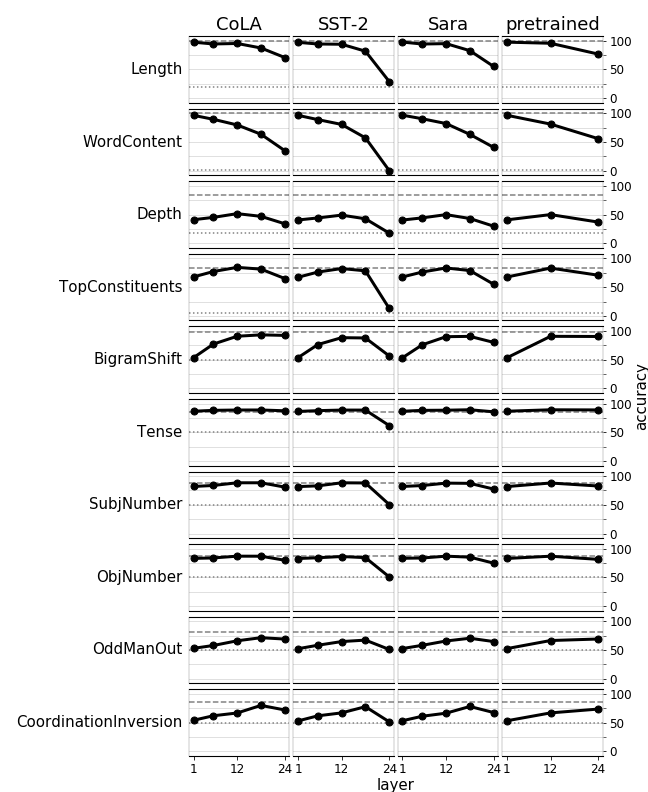
\includegraphics[width=12.5cm]{graphics/probing_master.png}
      \caption{Probing the 3 finetuned teachers and the pretrained one. The dotted line shows baseline accuracy levels achieved by majority-class guessing, the dashed line shows human performance.}
      \label{fig:probing-master}
    \end{figure}
  }
}

\chapter{Overall discussion and conclusions}{}

\chapter{Future work}{}

\chapter{Plan for the rest of the semester}{
  Work finished:
  \begin{itemize}
    \item implementing everything related to distillation (incl. teacher finetuning and generating augmentation data with GPT-2)
    \item creating augmented transfer sets and finetuning the BERT teacher for each task
    \item exploring the model parameters shared across tasks (i.e. doesn't include embedding type and student size)
    \item implementing everything needed for probing
    \item implementing everything needed for gathering predictions for mistake/confidence analysis
  \end{itemize}

  Work to be done:
  \begin{itemize}
    \item now-Feb 10: finishing size exploration for SST-2 and Sara (ending up with best students for each downstream task)
    \item Feb 11-23: analysing the predictions of all models (includes Inovative Learning Week Feb 17-21 when I won't get terribly much done)
    \item Feb 11-16: probing the best students
    \item Feb 24-Mar 1: putting together overall analysis and conclusions
    \item Mar 2-Apr 2: buffer time and writing the report (a lot of coursework in this period as well)
  \end{itemize}
}

% \chapter{Notes}{
%   \section{Knowledge distillation -- assorted}{
%     \citet{Zharov-et-al-2018} use KD of DNNs into decision forests for interpretability.
%   }

%   \section{Datasets}{
%     Unsuitable:
%     \begin{enumerate}
%       \item \href{https://github.com/microsoft/CNTK/tree/master/Examples/LanguageUnderstanding/ATIS}{ATIS}: too easy (see \href{https://github.com/nghuyong/rasa-nlu-benchmark#result}{here}). Rasa version \href{https://github.com/nghuyong/rasa-nlu-benchmark}{here}.
%       \item \href{https://github.com/sebischair/NLU-Evaluation-Corpora}{AskUbuntu, Chatbot and Web Applications (all from TU Munich): too small (max. 206 datapoints)}. Rasa version \href{https://github.com/nghuyong/rasa-nlu-benchmark}{here}.
%       \item \href{https://github.com/snipsco/nlu-benchmark/tree/master/2016-12-built-in-intents}{SNIPS}: too easy (see \href{https://github.com/nghuyong/rasa-nlu-benchmark#result}{here}). Rasa version \href{https://github.com/nghuyong/rasa-nlu-benchmark}{here}.
%     \end{enumerate}

%     Suitable:
%     \begin{enumerate}
%       \item \href{https://fb.me/multilingual_task_oriented_data}{FB's Multilingual Task Oriented Dataset}: F1 0.99 by supervised embeddings (very easy, but perhaps usable). Rasa version \href{https://github.com/nghuyong/rasa-nlu-benchmark}{here}.
%       \item \href{https://nyu-mll.github.io/CoLA/}{CoLA} \citep{CoLA-paper}, needs processing into Rasa format.
%       \item \href{https://nlp.stanford.edu/sentiment/index.html}{SST} \citep{SST-paper}, needs processing into Rasa format. 5-way classification may be too hard (accuracy \texttildelow{}50\%), 2-way much easier.
%       \item \href{https://cogcomp.seas.upenn.edu/Data/QA/QC/}{TREC question-type classification} \citep{TREC-paper}, needs processing into Rasa format. 6-way classification (abbreviation, entity, description, human, location, numeric), also has another (more fine-grained) level of categories.
%     \end{enumerate}

%     Maybe suitable:
%     \begin{enumerate}
%       \item \href{https://github.com/xiul-msr/e2e_dialog_challenge}{Microsoft Dialogue Challenge} \citep{MDC-paper} needs processing into Rasa format. Also, no results using Rasa.
%       \item \href{http://fb.me/semanticparsingdialog}{TOP} \citep{TOP-paper} needs processing into Rasa format. Also, no results using Rasa. Intents are hierarchical, would need to take only the top-most intent.
%       \item \href{https://github.com/allenai/scicite}{SciCite} \citep{SciCite-paper} needs processing into Rasa format. Also, no results using Rasa.
%     \end{enumerate}

%     Probing/evaluation:
%     Started by Shi et al. (2016) and Adi et al. (2017)?
%     \begin{enumerate}
%       \item \href{https://github.com/nyu-mll/jiant/tree/master/probing/data}{Google's edge probing} \citep{Tenney-et-al-2019-1} for evaluating span representations on 9 tasks closely following classical NLP pipeline (data not freely accessible!)
%       \item \href{https://github.com/facebookresearch/SentEval/tree/master/data/probing}{FB's probing} \citep{Conneau-et-al-2018} used to evaluate entire sentence embeddings (10 tasks from sentence length to semantics)
%       \item \href{https://github.com/facebookresearch/SentEval}{FB's SentEval} \citep{SentEval-paper} is meant for evaluating trained sentence encoders (i.e. not meant as downstream tasks that encoders should be fitted to), but it curates interesting existing datasets.
%     \end{enumerate}
%   }

%   \section{Plans for MVP}{
%     Let's distill BERT into a smaller BERT.

%     Code: pytorch-transformers (re-using code for DistilBERT), no Rasa for now.

%     Dataset: CoLA (because pytorch-transformers offers easy feeding of GLUE datasets).
%   }
% }

\bibliographystyle{apalike}
\bibliography{s1513472-minf2}

\appendix

\end{document}
